\documentclass[12]{thesis}
\bibliographystyle{unsrt}
%%% jdummy.def
%
\DeclareRelationFont{JY1}{mc}{it}{}{OT1}{cmr}{it}{}
\DeclareRelationFont{JT1}{mc}{it}{}{OT1}{cmr}{it}{}
\DeclareFontShape{JY1}{mc}{m}{it}{<5> <6> <7> <8> <9> <10> sgen*min
    <10.95><12><14.4><17.28><20.74><24.88> min10
    <-> min10}{}
\DeclareFontShape{JT1}{mc}{m}{it}{<5> <6> <7> <8> <9> <10> sgen*tmin
    <10.95><12><14.4><17.28><20.74><24.88> tmin10
    <-> tmin10}{}
\DeclareRelationFont{JY1}{mc}{sl}{}{OT1}{cmr}{sl}{}
\DeclareRelationFont{JT1}{mc}{sl}{}{OT1}{cmr}{sl}{}
\DeclareFontShape{JY1}{mc}{m}{sl}{<5> <6> <7> <8> <9> <10> sgen*min
    <10.95><12><14.4><17.28><20.74><24.88> min10
    <-> min10}{}
\DeclareFontShape{JT1}{mc}{m}{sl}{<5> <6> <7> <8> <9> <10> sgen*tmin
    <10.95><12><14.4><17.28><20.74><24.88> tmin10
    <-> tmin10}{}
\DeclareRelationFont{JY1}{mc}{sc}{}{OT1}{cmr}{sc}{}
\DeclareRelationFont{JT1}{mc}{sc}{}{OT1}{cmr}{sc}{}
\DeclareFontShape{JY1}{mc}{m}{sc}{<5> <6> <7> <8> <9> <10> sgen*min
    <10.95><12><14.4><17.28><20.74><24.88> min10
    <-> min10}{}
\DeclareFontShape{JT1}{mc}{m}{sc}{<5> <6> <7> <8> <9> <10> sgen*tmin
    <10.95><12><14.4><17.28><20.74><24.88> tmin10
    <-> tmin10}{}
\DeclareRelationFont{JY1}{gt}{it}{}{OT1}{cmbx}{it}{}
\DeclareRelationFont{JT1}{gt}{it}{}{OT1}{cmbx}{it}{}
\DeclareFontShape{JY1}{mc}{bx}{it}{<5> <6> <7> <8> <9> <10> sgen*goth
    <10.95><12><14.4><17.28><20.74><24.88> goth10
    <-> goth10}{}
\DeclareFontShape{JT1}{mc}{bx}{it}{<5> <6> <7> <8> <9> <10> sgen*tgoth
    <10.95><12><14.4><17.28><20.74><24.88> tgoth10
    <-> tgoth10}{}
\DeclareRelationFont{JY1}{gt}{sl}{}{OT1}{cmbx}{sl}{}
\DeclareRelationFont{JT1}{gt}{sl}{}{OT1}{cmbx}{sl}{}
\DeclareFontShape{JY1}{mc}{bx}{sl}{<5> <6> <7> <8> <9> <10> sgen*goth
    <10.95><12><14.4><17.28><20.74><24.88> goth10
    <-> goth10}{}
\DeclareFontShape{JT1}{mc}{bx}{sl}{<5> <6> <7> <8> <9> <10> sgen*tgoth
    <10.95><12><14.4><17.28><20.74><24.88> tgoth10
    <-> tgoth10}{}
\DeclareRelationFont{JY1}{gt}{sc}{}{OT1}{cmbx}{sc}{}
\DeclareRelationFont{JT1}{gt}{sc}{}{OT1}{cmbx}{sc}{}
\DeclareFontShape{JY1}{mc}{bx}{sc}{<5> <6> <7> <8> <9> <10> sgen*goth
    <10.95><12><14.4><17.28><20.74><24.88> goth10
    <-> goth10}{}
\DeclareFontShape{JT1}{mc}{bx}{sc}{<5> <6> <7> <8> <9> <10> sgen*tgoth
    <10.95><12><14.4><17.28><20.74><24.88> tgoth10
    <-> tgoth10}{}
\DeclareRelationFont{JY1}{gt}{it}{}{OT1}{cmr}{it}{}
\DeclareRelationFont{JT1}{gt}{it}{}{OT1}{cmr}{it}{}
\DeclareFontShape{JY1}{gt}{m}{it}{<5> <6> <7> <8> <9> <10> sgen*goth
    <10.95><12><14.4><17.28><20.74><24.88> goth10
    <-> goth10}{}
\DeclareFontShape{JT1}{gt}{m}{it}{<5> <6> <7> <8> <9> <10> sgen*tgoth
    <10.95><12><14.4><17.28><20.74><24.88> tgoth10
    <-> tgoth10}{}
\endinput
%%%% end of jdummy.def

 				% フォント関連のエラー対策(らしい)
\usepackage[dvipdfmx]{graphicx}
\usepackage{amsmath}			% math系
\usepackage{amssymb}			% math系
%\usepackage{float}				% 図表の挿入箇所を固定する[H]指定
\usepackage{cite}				% 参考文献
%\usepackage{url}				% 参考文献中のURL表記
\usepackage{algorithm}			% アルゴリズム環境
\usepackage{algorithmic}			% アルゴリズム環境
\usepackage{comment}			% コメントアウト環境
\usepackage{bm}					%太字形式のベクトル
\usepackage{amsthm}			%定理用?

%%% 泉先生がコメントをつける用 %%%
\usepackage[normalem]{ulem}
\usepackage{color}
\newcommand{\Izumi}[1]{\textcolor{blue}{#1}}
\newcommand{\Izurep}[2]{\textcolor{red}{\sout{#1}}{\Izumi{#2}}}

\headsep=1.4cm  %本文上にスペースを空けたい場合は 20mm にする

% 定理環境
\usepackage{amsthm} %定理用
\theoremstyle{definition}
\newtheorem{theorem}{定理}[chapter]
\newtheorem{lemma}{補題}[chapter]
\newtheorem{definition}{定義}[chapter]
\newtheorem{fact}{事実}[chapter]
\newtheorem*{prf*}{証明}
%\renewcommand{\theproof}{}
%\newcommand{\qed}{\hfill$\square$\par}

%%%%%%%% ここから本体 %%%%%%%%%%%%%%%%%%%%%%%%

\begin{document}
\baselineskip=22pt
\pagestyle{empty}

% タイトル
%\gradyear{2020}
\papertitleJP{$k$-極大独立集合検証問題の \\ 分散計算複雑性}
\papertitleEN{Distributed Complexity of k-Maximal \\ Independent Set Verification}
\studentID{31414050}
\degree{master}
\program{cs}
\labo{片山・金}
\enteryear{2019}
\name{佐藤 僚祐}
\maketitle

% 目次
\pagestyle{myheadings}	% ページ番号を右上につける
\pagenumbering{roman}	% ページ番号をローマ数字で
\tableofcontents

\newpage

% 本文
\pagenumbering{arabic}	% ページ番号をアラビア数字で

\chapter{はじめに}

\section{研究背景}
分散グラフアルゴリズムとは,計算機を頂点,辺を通信リンクとみなしてネットワークをモデル化したグラフ上において,
そのネットワーク自身を入力として様々な問題を解く枠組みである.分散アルゴリズムにおける代表的なモデルの
ひとつとして$CONGEST$モデルが存在する.$CONGEST$モデルにおいて,各ノードは同期して同じアルゴリズムを
実行して入力グラフ上の問題を解決する.各ノードは各ラウンドで(i)$b$ビットのメッセージを隣接ノードに送信
(ii)隣接ノードからメッセージを受信(iii)内部計算の3つの動作をする.標準的には,$b = \log n$を想定する.
$CONGEST$モデルにおいて,ある1つのノードにグラフ全体のトポロジの情報を集め,そのノード上で
逐次アルゴリズムを実行するという素朴なアプローチから自明に$O (n^{2})$ラウンドの上界を得ることができる.
$CONGEST$モデルにおける下界の証明では,下界をこの$n^{2}$にどれだけ近づけることができるかに興味がもたれている.

ネットワーク上の最大独立集合を発見する最大独立集合問題に対する数多くの分散グラフアルゴリズムが
研究されている.
%各頂点が隣接していない頂点部分集合を独立集合といい,最大独立集合とは頂点数が最も多い独立集合である.
大きなサイズの独立集合は経済学,計算生物学,符号理論,実験計画法など様々な分野への応用に用いられる \cite{kawarabayashi2019improved} が,そもそも最大独立集合問題はNP完全であり,頂点数$n$に対して
$n$の多項式時間で解くことは,その近似を含めて絶望的であるとされている.内部計算に指数時間かかることを
許した$CONGEST$モデルの下でラウンド数を$n$の多項式でおさえるような最大独立集合問題の複雑性の結果は
いくつか知られている \cite{kawarabayashi2019improved},  \cite{efron2020beyond}が,
内部計算に指数時間かかることを許容して分散グラフアルゴリズムの複雑性の議論を行うことの妥当性には
やや疑問が残る.そこで今回,我々は最大独立集合の局所最適解である$k$-極大独立集合
($k$-Maximal Independet Set, $k$-MIS)について考える.
%独立集合のうち,$k$個の頂点をその集合から取り除いて独立集合を維持したまま$k + 1$個以上の頂点を
%追加することができないとき,その独立集合を$k$-MISといい,
ネットワーク上の$k$-MISを発見する$k$-MIS問題は集中型アルゴリズムによって$O(n^{k + 2})$時間で
解くことができ,$k = O(1)$のとき$n$の多項式時間になるため,上記の疑問点を解決することができる.

今回は$k$-MISの検証問題(verification)に着目し,その複雑性について議論を行う.
$k$-MIS検証問題とはネットワーク上に独立集合が与えられ,それが$k$-MISかどうかを判定する問題である.
$k$-MIS問題に対する素朴な局所探索アルゴリズムは,ある1つの独立集合からスタートし, \\
(I)現在の状態が$k$-MISであるか判定. \\
(II)yesであればそれを出力,noであれば解を更新 \\
というフェーズを繰り返す.$k$-MIS検証問題は上記の(I)に対応しており,$k$-MIS問題と関連付いた問題ととらえることができる.

今回,我々は極大独立集合検証問題に対するいくつかの複雑性を示した.
最初に,1-MIS検証問題が$O(1)$ラウンドで解けることを証明した.
次に,2-MIS検証問題に対する$\tilde{\Omega} (\sqrt{n})$ラウンドの下界と
3-MIS検証問題に対する$\tilde{\Omega} (n)$ラウンドの下界を証明した.
最後に,$k$-MIS検証問題($k = 4l + 5, l \geq 1$)に対する$\tilde{\Omega} (n^{2 - \frac{1}{l + 1}})$ラウンドの下界を証明した.
特に,下界の証明のアイデアは2者間通信の枠組みにおける交叉判定問題からの帰着に基づいている.

\section{関連研究} %途中
$CONGEST$モデルにおける最大独立集合問題の通信複雑性としては,頂点の最大次数を$\Delta$としたとき,
最大重み付き独立集合の$(1 + \epsilon) \cdot \Delta$-近似を高確率で見つけるアルゴリズムに対する
$(\frac{poly(\log \log n)}{\epsilon})$ラウンドの上界 \cite{kawarabayashi2019improved} や,
最大独立集合の$(\frac{1}{2} + \epsilon)$-近似を見つけるアルゴリズムに対する
$\Omega (\frac{n}{(\log n)^{3}})$ラウンドの下界,$(\frac{3}{4} + \epsilon)$-近似を見つけるアルゴリズムに対する
$\Omega (\frac{n^{2}}{(\log n)^{3}})$ラウンドの下界 \cite{efron2020beyond} が知られている.
 
本研究の下界に関する結果は2者間通信の枠組みにおける交叉判定問題からの帰着に基づいているが,
交叉判定問題からの帰着によって下限を示すという証明方法は多くの問題に対して用いられている.例えば,
最小カット発見 \cite{ghaffari2013distributed} や部分グラフ検出 \cite{fischer2018possibilities} ,
近似最大クリーク検出 \cite{czumaj2020detecting} といったさまざまな問題に対する下界の証明がされている.

\section{本研究の成果}
今回,我々は極大独立集合検証問題に対するいくつかの複雑性を示した.
最初に,1-MIS検証問題が$O(1)$ラウンドで解けることを証明した.
次に,2-MIS検証問題に対する$\tilde{\Omega} (\sqrt{n})$ラウンドの下界と
3-MIS検証問題に対する$\tilde{\Omega} (n)$ラウンドの下界を証明した.
最後に,$k$-MIS検証問題($k = 4l + 5, l \geq 1$)に対する$n^{2 - \frac{1}{l + 1}}$ラウンドの下界を証明した.

\section{論文の構成}
本論文は全5章で構成される.第2章ではグラフの構造と用語の定義をしている.
第3章では1-MIS検証問題に対する$O(1)$ラウンドアルゴリズムについて述べている.
第4章ではk-MIS検証問題($k = 2, 3, 4l + 5( l \geq 1)$)に対する下界について述べている.
第5章ではまとめについて述べている.

\chapter{諸定義}

\subsection*{$CONGEST$モデル}
本稿で考える$CONGEST$モデルは,単純無向グラフ連結グラフ$G = (V, E)$により表現される.ここで$V$はノードの集合で
$|V| = n$とし,$E$は通信リンクの集合である.$CONGEST$モデルでは計算機はラウンドに従って同期して動作するものとする.
1ラウンド内で,隣接頂点へのメッセージ送信,隣接頂点からのメッセージ受信,内部計算を行う.各辺は単位ラウンドあたり
$b$ビットを双方向に伝送可能であり,各ノードは同一ラウンドに異なる接続辺に異なるメッセージを送信可能である.
標準的には,$b = \log n$を想定する.また,各ノードには$O(\log n)$ビットの自然数値によるIDが付与されており,
自身の隣接ノードすべてのIDを既知であるとする.各ノードはグラフのトポロジに関する事前知識を持たないものとする.

\subsection*{2者間通信複雑性}
2者間通信複雑性の枠組みでは,アリスとボブの二人のプレイヤーがそれぞれ$k$ビットの0/1のデータ列で構成される
プライベートな入力$x$および$y$を持っているとする.プレイヤーの目標は,結合関数$f(x, y)$を計算することであり,
複雑性の尺度として$f(x, y)$を計算するためにアリスとボブが通信によって交換する必要のあるビット数が用いられる.

この枠組みにおける重要な問題として,交叉判定問題(set-disjointness)がある.この問題では,アリスとボブは
それぞれ$x \in \{0, 1\}^{k}$と$y \in \{0, 1\}^{k}$を入力として持ち,目的は
$DISJ_{k} (x, y) :=\bigvee_{i = 1}^{k} x_{i} \land y_{i}$を計算することである.$k$ビットの交叉判定問題を解くために,
アリスとボブは通信によって$\Omega (k)$ビット交換する必要があることが知られており 
\cite{kalyanasundaram1992probabilistic},この事実を用いて最小カット発見 \cite{ghaffari2013distributed} や
部分グラフ検出 \cite{fischer2018possibilities} ,近似最大クリーク検出 \cite{czumaj2020detecting} といった
さまざまな問題に対する下界の証明がされている.

$CONGEST$モデルにおいて,入力グラフ上に特性$P$があるかどうかの判定に対する下限の証明を
2者間交叉判定問題から帰着するアプローチは以下のとおりである.
最初にアリスとボブは特殊なグラフ$G = (V, E)$の構築と$G$を$G_{A}$と$G_{B}$に分割するカット辺$C$の決定を行う.
次に,アリスとボブは入力文字列に基づいてそれぞれ$G_{A}$と$G_{B}$に辺$E_{A}$と$E_{B}$を追加する.
このとき,$DISJ_{k} (x, y)=1$のときのみ,何らかの特性$P$(例えば,$P$:「グラフに与えられたMISが2-MISでない」)を持つように
辺を追加する.また,カット辺$C$は入力文字列に依存しないようにする.グラフ$G$に辺を追加したグラフを$G' = (V', E')$とすると
$V' = V, E' = E \cap (E_{A} \cap E_{B})$表すことができる.グラフ$G'$の構造の概要を図 \ref{Dif_Gx} に示す.

\begin{figure}[ht]
\begin{center}
\includegraphics[width=120mm]{Dif_Gx.png}
\end{center}
\caption{G' = (V, E')}
\label{Dif_Gx}
\end{figure}

アリスとボブは,入力グラフ上に特性$P$があるかを判定する分散アルゴリズムをシミュレートできる.
2者間通信複雑性モデルでのシミュレートは,次のように実行される.$G_{A}$中の辺で送信されるメッセージ,あるいは
$G_{B}$中の辺で送信されるメッセージは,アリスとボブがそれぞれお互いと通信せずにシミュレートできる.カット辺$C$を通じて
送信されるメッセージに対しては,お互い情報を交換する必要がある.$CONGEST$モデルにおいてグラフ上に特性$P$が
あるかどうかを$r$ラウンドで判定するアルゴリズム$\mathcal{A}$が存在したとすると,アリスとボブは特性$P$の判定のために
$O(r \cdot |C| \cdot b)$ビット通信したことになる.これは,各ラウンドで,アルゴリズムが各辺で$O(b)$ビットの通信を
行っているからである.このグラフにおいてアルゴリズム$\mathcal{A}$を実行すると同時に2者間交叉判定問題も解けていることになる.例えばアルゴリズムを実行した結果,入力グラフに特性$P$があると判定されれば$DISJ_{k} (x, y)=1$であるとわかるからである.
交叉判定問題の通信複雑性よりアリスとボブは少なくとも$\Omega (k)$ビットは通信しているはずである.
したがって,$CONGEST$モデルにおいてと特性$P$があるかどうかを判定する任意のアルゴリズムに対して
$r = \Omega (k / |C| \cdot b)$ラウンドの下界を得ることができる.カット辺の大きさが小さくなるほど下界が強くなる.

\subsection*{$k$-極大独立集合}
\begin{definition}
$I$が$k$-極大独立集合 $ \Leftrightarrow$ \\
\begin{math}
\lnot \left( \exists I' \subseteq I |I'| = k,  \\ \exists S \subseteq V |S|\geq k + 1, (I\setminus I')\cap Sが独立集合 \right)
\end{math}
\end{definition}
つまり,ある独立集合$I$に対して,サイズ$k$の$I$の部分集合$I'$を取り除いてサイズ$k + 1$以上の$V$の部分集合$S$をくっつけたものが新たな独立集合になり得ないとき,$I$を$k$-MISと定義する.

\newpage

\chapter{1-MIS検証問題の1ラウンドアルゴリズム}
ddddd

\chapter{$k$-MIS検証問題の下限}
この章では,MIS検証問題の下界についての議論を行う.
4.1節では,2-MIS検証問題の下界についての定理とその証明を述べる.
4.2節では,3-MIS検証問題の下界についての定理とその証明を述べる.
4.3節では,$k$-MIS検証問題($k = 4l + 5, l \geq 1$)の下界についての定理とその証明を述べる.

\section{2-MIS検証問題の下限}
この節では2-MIS検証問題の下界についての議論を行う.具体的には,次の定理を証明する. 
\begin{theorem}
$CONGEST$モデルにおいて,2-MIS検証問題を解く全てのアルゴリズムは$\tilde{\Omega} (\sqrt{n})$の通信ラウンド数を必要とする.
\end{theorem}
\begin{prf*}
まず初めにアリスとボブが構築するグラフ$G' = (V', E')$を図 \ref{2MIS}に示す. 

\begin{figure}[ht]
\begin{center}
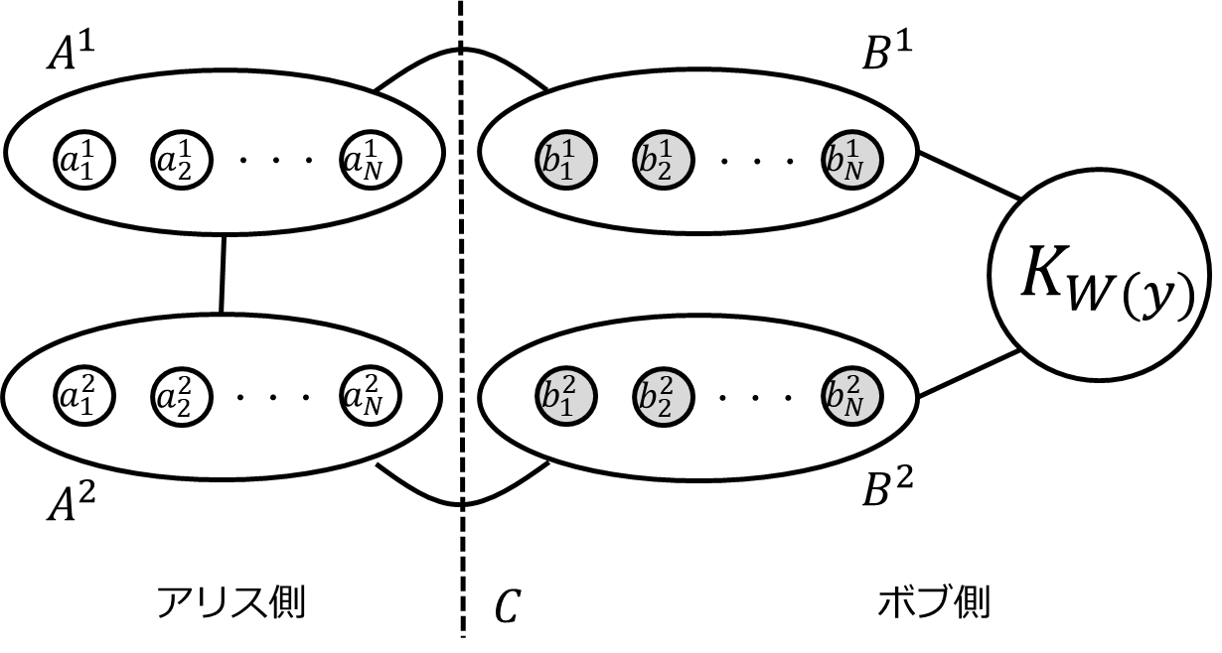
\includegraphics[width=120mm]{2MIS.png}
\end{center}
\caption{G' = (V, E')}
\label{2MIS}
\end{figure}

図中の頂点のうち,灰色のものは独立集合に含まれる頂点とする.図中で省略されている辺と$K_{W(y)}$の構造は次のとおりである.
\begin{itemize}
%\item $A^{1}, A^{2}, B^{1}, B^{2}$は$N$頂点のクリーク$K_{N}$
%\item $\forall i, j((a_{i}^{1}, a_{j}^{1}), (a_{i}^{2}, a_{j}^{2}), (b_{i}^{1}, b_{j}^{1}), (b_{i}^{2}, b_{j}^{2})) \in E$
\item $\forall i((a_{i}^{1}, b_{i}^{1}), (a_{i}^{2}, b_{i}^{2})) \in E$
%\item $\forall i((a_{i}^{1}, s), (a_{i}^{2}, s), (b_{i}^{1}, s), (b_{i}^{2}, s)) \in E$
\item $(a_{i}^{1}, a_{j}^{2}) \in E_{A} \Leftrightarrow x_{i, j} = 0$
\item $W(y)$は0/1のデータ列$y$中に含まれる1の個数を表す.
$K_{W(y)}$中の頂点$c_{i, j}$は$y_{i, j} = 1$であるような$(i, j)$でインデックスづけされるものとする. \\
このとき,$(c_{i, j}, b_{i}^{1}) \in E_{B}$ かつ $(c_{i, j}, b_{j}^{2}) \in E_{B}$
\end{itemize}

このグラフは,「$G'$中に与えられている独立集合が,$DISJ_{N \times N} (x, y) = 1$のときのみ2-MISでない」という特性を持つ. 
(なお,$DISJ_{N \times N} (x, y) :=\bigvee_{i = 1}^{N} \bigvee_{j = 1}^{N} x_{i, j} \land y_{i, j}$で定義される.)
このグラフが上記の特性を満たしていることを示すために,次の2点を確認する. \\
(i)$DISJ_{N \times N} (x, y) = 1$のとき,グラフに与えられている独立集合が2-MISでない: \\
$x_{i, j} = y_{i, j} =1$とすると,$b_{i}^{1}$と$b_{j}^{2}$の2点を取り除いて$a_{i}^{1}$, $a_{j}^{2}$, $c_{i, j}$の
3点を追加できることから確認できる. \\
(ii)$DISJ_{N \times N} (x, y) = 0$のとき,グラフに与えられている独立集合が2-MISである: \\ 
グラフに与えられている独立集合が2-MISでないと仮定する.このとき,ある2点を取り除くことで独立集合に追加できる3点が存在する.
2点の取り除き方は(1)$b_{i}^{1}$と$b_{j}^{1}(i \neq j)$, (2)$b_{i}^{2}$と$b_{j}^{2}(i \neq j)$, (3)$b_{i}^{1}$と$b_{j}^{2}$が考えられる.
(1)では$a_{i}^{1}$と$a_{j}^{1}$の2点しか追加できる可能性がなく,(2)では$a_{i}^{2}$と$a_{j}^{2}$の2点しか追加できる可能性がない.
(3)において,$b_{i}^{1}$を取り除いて$a_{i}^{1}$を追加し,$b_{j}^{2}$を取り除いて$a_{j}^{2}$を追加し,さらに$c_{i, j}$を追加することを考える.
$a_{i}^{1}$と$a_{i}^{2}$が両方とも追加できるのは$x_{i, j} = 1$のときのみであり,$c_{i, j}$が追加できる($c_{i, j}$が存在する)のは
$y_{i, j} = 1$のときのみであるが,これは$DISJ_{N \times N} (x, y) = 0$に矛盾する.したがってグラフに与えられている独立集合から2点取り除いて
3点追加することはできないため,この独立集合は2-MISである.

今回,$N \times N$ビットの交叉判定インスタンスをグラフに埋め込んでおり,カット辺のサイズ$|C| = 2N$であることがわかる.
$CONGEST$モデルにおいてグラフ上に与えられた独立集合が2-MISであるかどうかを$r$ラウンドで判定する
アルゴリズム$\mathcal{A}$が存在したとすると,アリスとボブは$O(r \cdot |C| \cdot b)$ビット通信したことになる.
このグラフにおいてアルゴリズム$\mathcal{A}$を実行すると同時に2者間交叉判定問題も解けていることになるので,
交叉判定問題の通信複雑性よりアリスとボブは少なくとも$\Omega (N \times N)$ビットは通信しているはずである.
よって,$r = \Omega (N / 2b) = \tilde{\Omega}(N)$ラウンドの下界を得ることができる.図\ref{2-MIS}からわかる通り,
$A^{1}, A^{2}, B^{1}, B^{2}$は$N$頂点で構成されており,$K_{W(y)}$の頂点数は$O(N^{2})$であるため,
グラフ全体の頂点数$n$は$n = O(N + N^{2})$である.したがって$N = O(\sqrt{n})$になるため,
$\tilde{\Omega}(\sqrt{n})$ラウンドの下界を得ることができる. 
\end{prf*}
\newpage

\section{3-MIS検証問題の下限}
この節では3-MIS検証問題の下界についての議論を行う.具体的には,次の定理を証明する.
\begin{theorem}
$CONGEST$モデルにおいて,3-MIS検証問題を解く全てのアルゴリズムは$\tilde{\Omega} (n)$の通信ラウンド数を必要とする.
\end{theorem}

\begin{prf*}
まず初めにアリスとボブが構築するグラフ$G' = (V', E')$を図 \ref{3MIS}に示す. 

\begin{figure}[ht]
\begin{center}
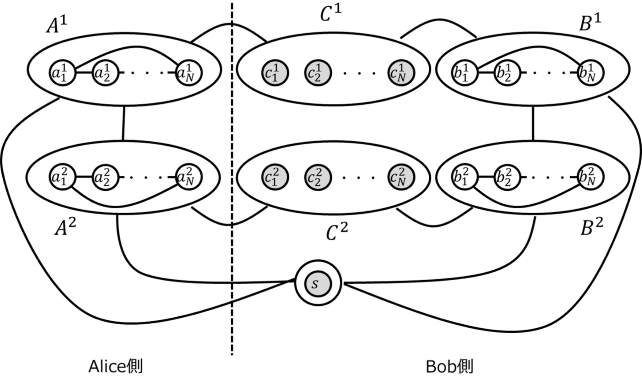
\includegraphics[width=120mm]{3MIS.png}
\end{center}
\caption{G' = (V, E')}
\label{3MIS}
\end{figure}

図中の頂点のうち,灰色のものは独立集合に含まれる頂点とする.図中で省略されている辺は次のとおりである.
\begin{itemize}
\item $A^{1}, A^{2}, B^{1}, B^{2}$は$N$頂点のクリーク$K_{N}$
%\item $\forall i, j((a_{i}^{1}, a_{j}^{1}), (a_{i}^{2}, a_{j}^{2}), (b_{i}^{1}, b_{j}^{1}), (b_{i}^{2}, b_{j}^{2})) \in E$
\item $\forall i((a_{i}^{1}, c_{i}^{1}), (a_{i}^{2}, c_{i}^{2}), (b_{i}^{1}, c_{i}^{1}), (b_{i}^{2}, c_{i}^{2})) \in E$
\item $\forall i((a_{i}^{1}, s), (a_{i}^{2}, s), (b_{i}^{1}, s), (b_{i}^{2}, s)) \in E$
\item $(a_{i}^{1}, a_{j}^{2}) \in E_{A} \Leftrightarrow x_{i, j} = 0$, $(b_{i}^{1}, b_{j}^{2}) \in E_{B} \Leftrightarrow y_{i, j} = 0$
\end{itemize}

このグラフは,「$G'$中に与えられている独立集合が,$DISJ_{N \times N} (x, y) = 1$のときのみ3-MISでない」という特性を持つ. 
このグラフが上記の特性を満たしていることを示すために,次の2点を確認する. \\
(i)$DISJ_{N \times N} (x, y) = 1$のとき,グラフに与えられている独立集合が3-MISでない: \\
$x_{i, j} = y_{i, j} =1$とすると,$s$と$c_{i}^{1}$と$c_{j}^{2}$の3点を取り除いて$a_{i}^{1}$, $b_{i}^{1}$, $a_{j}^{2}$, $c_{j}^{2}$の
4点を追加できることから確認できる. \\
(ii)$DISJ_{N \times N} (x, y) = 0$のとき,グラフに与えられている独立集合が3-MISである: \\ 
グラフに与えられている独立集合が3-MISでないと仮定する.このとき,ある3点を取り除くことで独立集合に追加できる4点が存在するが,
$A^{1}, A^{2}, B^{1}, B^{2}$がそれぞれクリークであるため,4点を追加するためにはそれぞれから1点を選ぶ必要がある.
$c_{i}^{1}$を取り除いて$a_{i}^{1}$と$b_{i}^{1}$を追加し,,$c_{j}^{2}$を取り除いて,$a_{j}^{2}$と$b_{j}^{2}$を独立集合に追加したとする.
$a_{i}^{1}$と$a_{i}^{2}$が両方とも追加できるのは$x_{i, j} = 1$のときのみであり,$b_{i}^{1}$と$b_{i}^{2}$が両方とも追加できるのは
$y_{i, j} = 1$のときのみであるが,これは$DISJ_{N \times N} (x, y) = 0$に矛盾する.したがってグラフに与えられている独立集合から3点取り除いて
4点追加することはできないため,この独立集合は3-MISである.

今回,$N \times N$ビットの交叉判定インスタンスをグラフに埋め込んでおり,カット辺のサイズ$|C| = 4N$であることがわかる.
$CONGEST$モデルにおいてグラフ上に与えられた独立集合が3-MISであるかどうかを$r$ラウンドで判定する
アルゴリズム$\mathcal{A}$が存在したとすると,アリスとボブは$O(r \cdot |C| \cdot b)$ビット通信したことになる.
このグラフにおいてアルゴリズム$\mathcal{A}$を実行すると同時に2者間交叉判定問題も解けていることになるので,
交叉判定問題の通信複雑性よりアリスとボブは少なくとも$\Omega (N \times N)$ビットは通信しているはずである.
よって,$r = \Omega (N / 4b) = \tilde{\Omega}(N)$ラウンドの下界を得ることができる.図\ref{3-MIS}からわかる通り,
$A^{1}, A^{2}, B^{1}, B^{2}, C^{1}, C^{2}$は$N$頂点で構成されているため,グラフ全体の頂点数$n$は$n = O(N)$である.
したがって$N = O(n)$になるため,$\tilde{\Omega}(n)$ラウンドの下界を得ることができる. 
\end{prf*}
\newpage

\section{$k$-MIS検証問題の下限}
このセクションではk-MIS検証問題の下界についての議論を行う.具体的には,次の定理を証明する.

\newpage

\chapter{まとめと今後の課題}
\section{まとめ}
本研究では極大独立集合検証問題に対するいくつかの複雑性を示した.
具体的には,1-MIS検証問題に対する$O(1)$ラウンドの上界,
2-MIS検証問題に対する$\tilde{\Omega} (\sqrt{n})$ラウンドの下界
3-MIS検証問題に対する$\tilde{\Omega} (n)$ラウンドの下界,.
$k$-MIS検証問題($k = 4l + 5, l \geq 1$)に対する$n^{2 - \frac{1}{l + 1}}$ラウンドの下界を証明した.

\section{今後の課題}
4.3節で一般の$k$に対する$k$-MIS検証問題の下界を証明したが,$k = 4,...,8$については現在
3-MIS検証問題と同じ下界しか得られていない.この下界をよりタイトにできるかが今後の課題である.
\newpage

\chapter*{謝辞}
本研究の機会を与え,数々の御指導を賜りました泉泰介准教授に深く感謝致します.
また,本研究を進めるにあたり多くの助言を頂き,様々な御協力を頂きました泉研究室
の学生のみなさんに深く感謝致します.

\newpage

\bibliography{M2sato}

%ここから下は卒論のコピペだから関係ない
\begin{comment}

\section{関連研究}
最大$k$-plex問題を解くためのアルゴリズムとして,以下のようなものが研究されている.
\begin{itemize}
 \item 最大$k$-plex問題を整数計画法で定式化してbranch-and-cutを
	用いるアルゴリズムの研究 \cite{balasundaram2011clique}
 \item グラフ彩色問題の概念を一般化して$k$-plexの基数の上限を導いて
	それを利用した組み合わせアルゴリズムの研究 \cite{mcclosky2012combinatorial}
 \item 最大$k$-plex問題と双対性を持つ$d$-BDD(Bounded-Degree-$d$ Vertex Detection)問題の
	解を見つけるアルゴリズムの研究 \cite{moser2012exact}
\end{itemize}
上記の研究で提案されている最大$k$-plex問題を解くためのアルゴリズムは
全て$2^{n}n^{O(1)}$時間で動く.

また,複数のブランチングルールを持ったbranch-and-searchアルゴリズムによって
最大$k$-plex問題を$\sigma_{k}^{n}n^{O(1) }$ ($\sigma_{k} < 2$は$k$に関する値)で解く
アルゴリズムがある.これは$2^{n}$という理論的限界を破った最初のアルゴリズムである. \cite{xiao2017fast} 

\begin{lemma} \label{lemma:3}
$S$を$k$-plexの頂点集合とする.ある頂点$v$が$S$に含まれているとき,
$v$から距離が2以上離れた頂点は$k$つ以上$S$に含まれない.
\begin{prf*}
$v$は2-plexの頂点集合$S$に含まれているとする.$v$から距離2以上離れた$k$頂点
$a_{1}, a_{2}, \dots, a_{k}$が全て$S$に含まれていると仮定する.$k$-plexの定義より,
$S$中に含まれる全ての頂点は少なくとも$|S| - k$の次数を持つ,つまり$S$中に含まれる
頂点は$S$中の$|S| - k$頂点と隣接しているはずである.
しかし$v$は$v, a_{1}, a_{2}, \dots, a_{k}$の$k + 1$頂点と隣接していないので,矛盾する.
したがって$a_{1}, a_{2}, \dots, a_{k}$は全て$S$に含まれることはない.
\end{prf*}
\end{lemma}

%ここらへん曖昧
これらの補題をふまえ,最大$k$-plex問題に関する定理とその証明を示す.
\begin{theorem} \label{theorem:3}
$m$本の辺を持ったグラフの最大$k$-plex問題を
$O(n^{k}2^{\sqrt{m}})$時間で解くアルゴリズムが存在する.
\begin{prf*}
$G$を連結グラフとする.最小次数の頂点$v$を選ぶ.定理 \ref{theorem:1} と同様の議論により
$v$の次数は$\sqrt{m}$未満であるとする.

$G$中の最大サイズの$k$-plexである$S$を見つけるために2つの部分問題にブランチする.
\begin{enumerate}
 \item $v$が$S$中の頂点の1つである
 \item $v$が$S$中の頂点の1つでない
\end{enumerate}
1つ目の部分問題では$S$に含まれる可能性のある頂点部分集合を探索して
$v$を含んだ最大$k$-plexを見つける.
2つ目の部分問題では$v$を$G$から削除してアルゴリズムを再帰的に呼び出す.

このアルゴリズムのステップ数が多くとも$n^{k}2^{\sqrt{m}}$になることを$m$への帰納法によって証明する.
\begin{itemize}
 \item $m = 0$のとき,$G$はただ1つの$k$-plexを持ち,その大きさは1である.	
 \item $v \in C$の場合に対応した部分問題を解くために,$v$を含んだ最大サイズの$k$-plexである$S$を選ぶ.
補題  \ref{lemma:3} より,$v$から距離2以上離れている頂点は$k$つ以上は$S$に含まれない.
$v$の近傍の頂点数を$M$,$v$から距離2以上離れた頂点数を$N$とすると,$S$を選ぶのに必要な頂点数は
\[ 2^{M} \times  \sum_{i = 1}^{k - 1}\binom{N}{i}  \]
である.$M < \sqrt{m}$,$N \leqq n$ であり,また
\[ \sum_{i = 1}^{k}\binom{n}{i}  \leqq {\left( \frac{en}{k} \right)}^{k} \]
であることが知られているので必要なステップ数は多くとも${\left( \frac{en}{k} \right)}^{k}2^{\sqrt{m}}$ステップである.
 \item $v \notin C$の場合,帰納法の仮定によって問題は
多くとも$(n - 1){\left( \frac{en}{k} \right)}^{k}2^{\sqrt{m}}$ステップで解ける.
\end{itemize}
ゆえにアルゴリズムの合計のステップ数は
\[  {\left( \frac{en}{k} \right)}^{k}2^{\sqrt{m}} +  (n - 1){\left( \frac{en}{k} \right)}^{k}2^{\sqrt{m}} =n{\left( \frac{en}{k} \right)}^{k}2^{\sqrt{m}} \]
でありその実行時間は $O(n{\left( \frac{en}{k} \right)}^{k}2^{\sqrt{m}}) = O(n^{k}2^{\sqrt{m}})$である.
\end{prf*}
\end{theorem}

\newpage

\chapter{まとめと今後の課題}
\section{まとめ}
今回の研究では,既存の$2^{O(\sqrt{m})}$時間の最大クリーク問題のアルゴリズムを
応用して最大$k$-plexを解くアルゴリズムを考えた.その結果,最大$k$-plex問題を
$O(n^{k}2^{\sqrt{m}})$時間で解くアルゴリズムを得ることができた.このアルゴリズムは,
辺の本数に関するパラメータ$m$の準指数時間で動く.したがって,辺の本数が少ない,
密でないグラフに対して有効なアルゴリズムである.

\section{今後の課題}
補題  \ref{lemma:2} を応用すると,$v$から距離$k$より離れた点は最大$k$-plexの集合に
含まれないことが示せる. \ref{section:2plex} のアルゴリズムでは,最大$k$-plexの集合に
含まれることがない頂点も探索しているので,無駄が存在する.この無駄を解消するために,
頂点を$v$からの距離によって場合分けして探索範囲を減らすアルゴリズムを考えたが,
計算時間$O(n^{k}2^{\sqrt{m}})$の境界を破ることはできなかった.
$v$からの距離以外の別のアプローチによって$O(n^{k}2^{\sqrt{m}})$の境界を突破するとこが
今後の課題である.

\newpage

\chapter*{謝辞}
本研究の機会を与え,数々の御指導を賜りました泉泰介准教授に深く感謝致します.
また,本研究を進めるにあたり多くの助言を頂き,様々な御協力を頂きました泉研究室
の学生のみなさんに深く感謝致します.

\newpage

\bibliography{M2sato}

\subsection*{$k$-極大独立集合2}
\begin{definition}

\begin{figure}[ht]
\begin{center}
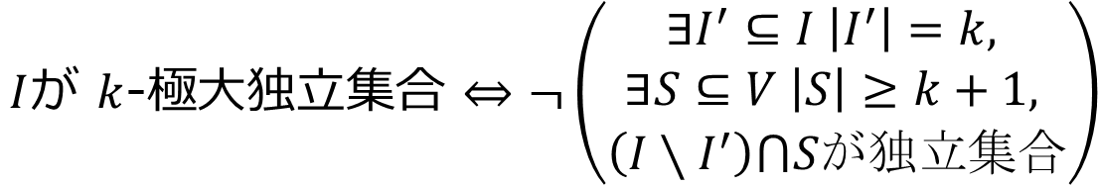
\includegraphics[width=120mm]{Dif_MIS.png}
\end{center}
\end{figure}

\end{definition}
つまりarufourusdafafsdadfaf$I$である.
\end{comment}

\end{document}